\documentclass[12pt]{article}

\usepackage{fixltx2e}
\usepackage{textcomp}
\usepackage{fullpage}
\usepackage{amsfonts}
\usepackage{verbatim}
\usepackage[english]{babel}
\usepackage{pifont}
\usepackage{color}
\usepackage{setspace}
\usepackage{lscape}
\usepackage{indentfirst}
\usepackage[normalem]{ulem}
\usepackage{booktabs}
% \usepackage{nag}
\usepackage{natbib}
% \usepackage{bibtex}
\usepackage{float}
\usepackage{latexsym}
\usepackage{hyperref}
\usepackage{url}
% \usepackage{html}
\usepackage{epsfig}
\usepackage{graphicx}
\usepackage{amssymb}
\usepackage{amsmath}
\usepackage{bm}
\usepackage{array}
%\usepackage{mhchem}
\usepackage{ifthen}
\usepackage{caption}
\usepackage{xcolor}
\usepackage{amsthm}
\usepackage{amstext}
\usepackage{nicefrac}
\usepackage{algorithm}
\usepackage{algorithmic}
\usepackage[scientific-notation=true]{siunitx}
\usepackage{subfigure}
\usepackage[flushleft]{threeparttable}
\usepackage{lineno}
\usepackage{adjustbox}

\begin{document}

\begin{minipage}[h]{\textwidth}
	\title{StarBEAST2 enables accurate and precise inference of species trees, divergence times and clock rates}
	\author{Huw A. Ogilvie$^{\ast,1,2}$ and Alexei J. Drummond,$^{2,3}$}
    \maketitle
\end{minipage}

\raggedright
$^{1}$Department of Evolution, Ecology and Genetics, Australian National University, Canberra, Australia\\
$^{2}$Centre for Computational Evolution, University of Auckland, Auckland, New Zealand\\
$^{3}$Department of Computer Science, University of Auckland, Auckland, New Zealand

\clearpage

\section{Abstract}

Keywords: Phylogenetic methods, substitution rate, relaxed clock, multispecies coalescent, concatenation.

\section{Introduction}


\section{New Approaches}


\section{Results}

\subsection{StarBEAST2 is validated by simulation}



\subsection{New operators and analytical integration improve computational performance}



\begin{figure}[htb!]
\centering
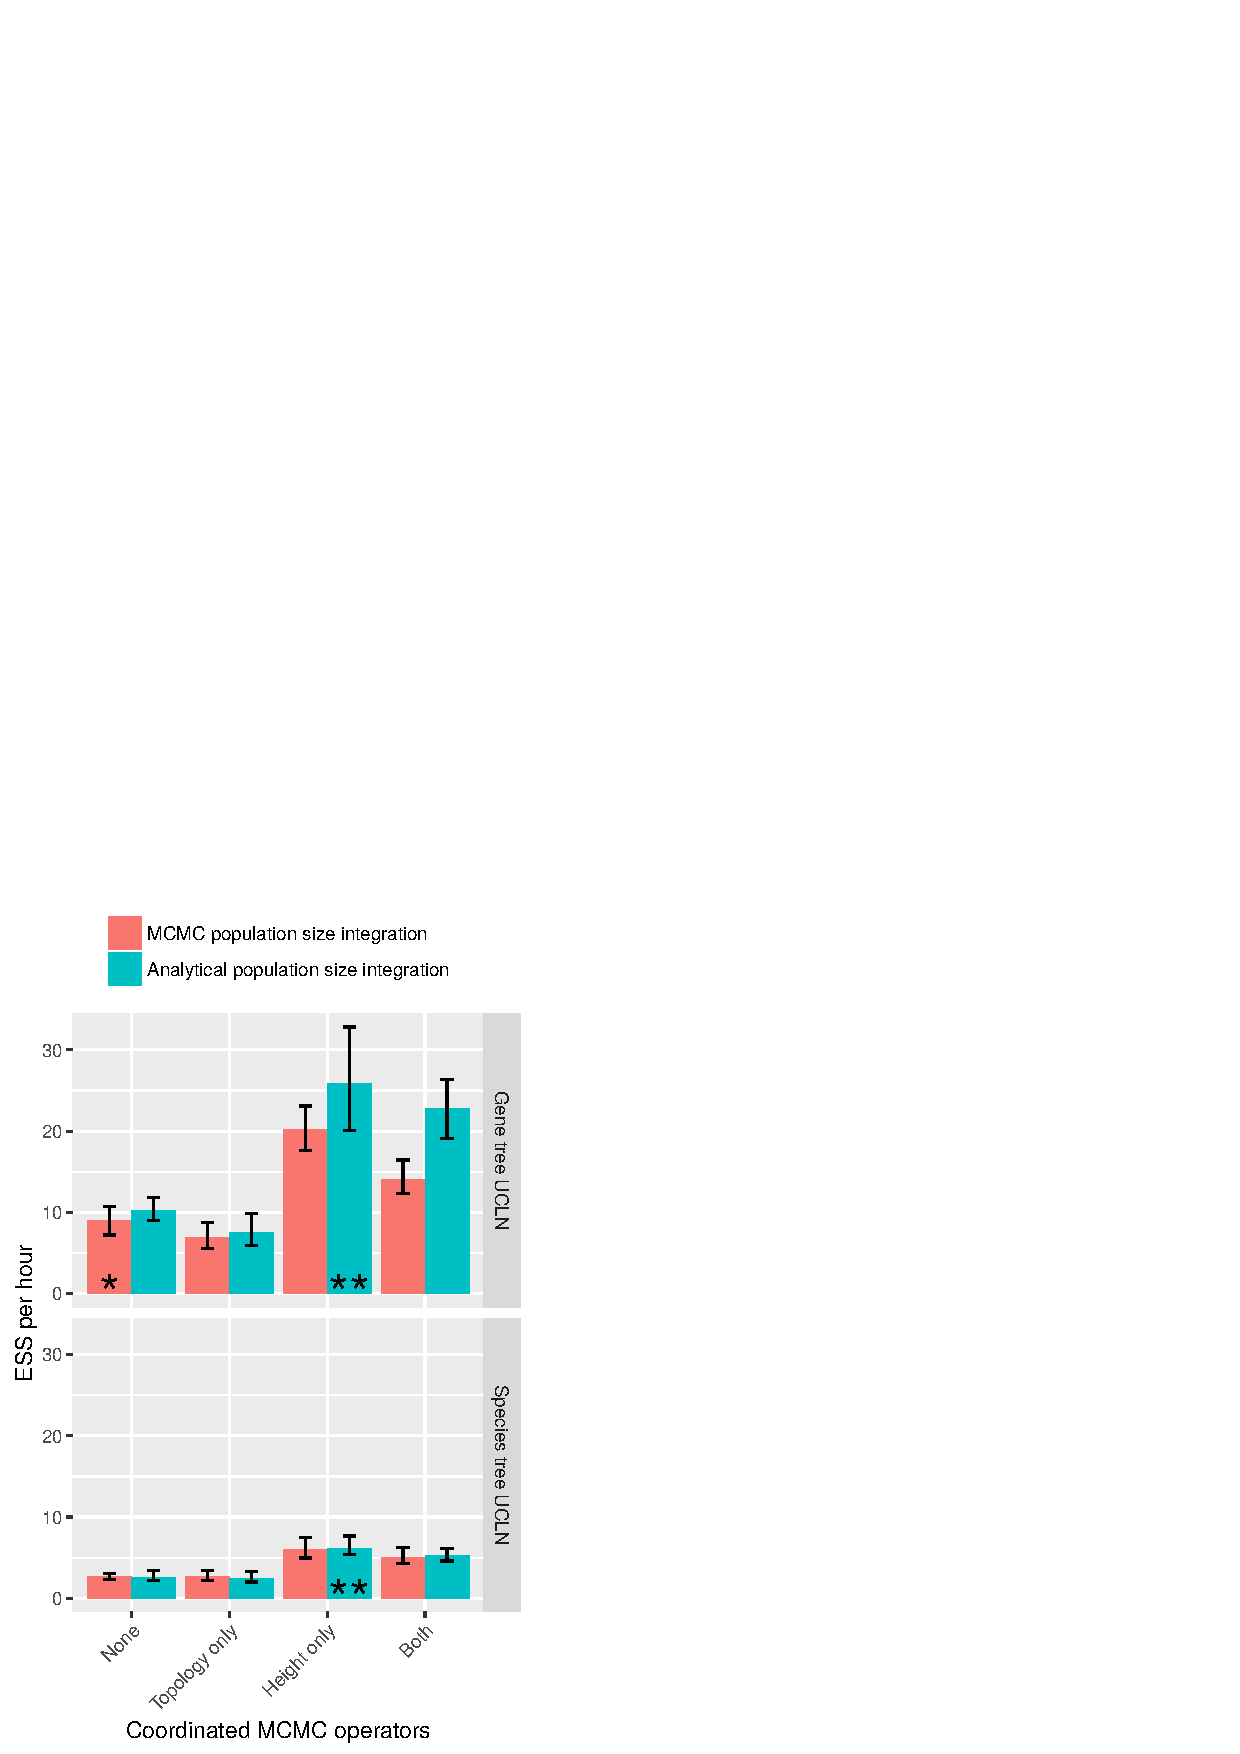
\includegraphics[height=14cm]{speciesTreeHeight_ess_per_hour.pdf}
\caption
{Mean estimated sample size (ESS) per hour of the \textit{Pseudacris} species tree height.}
\label{fig:realEssPerHour}
\end{figure}

\clearpage

\begin{figure}[htb!]
\centering
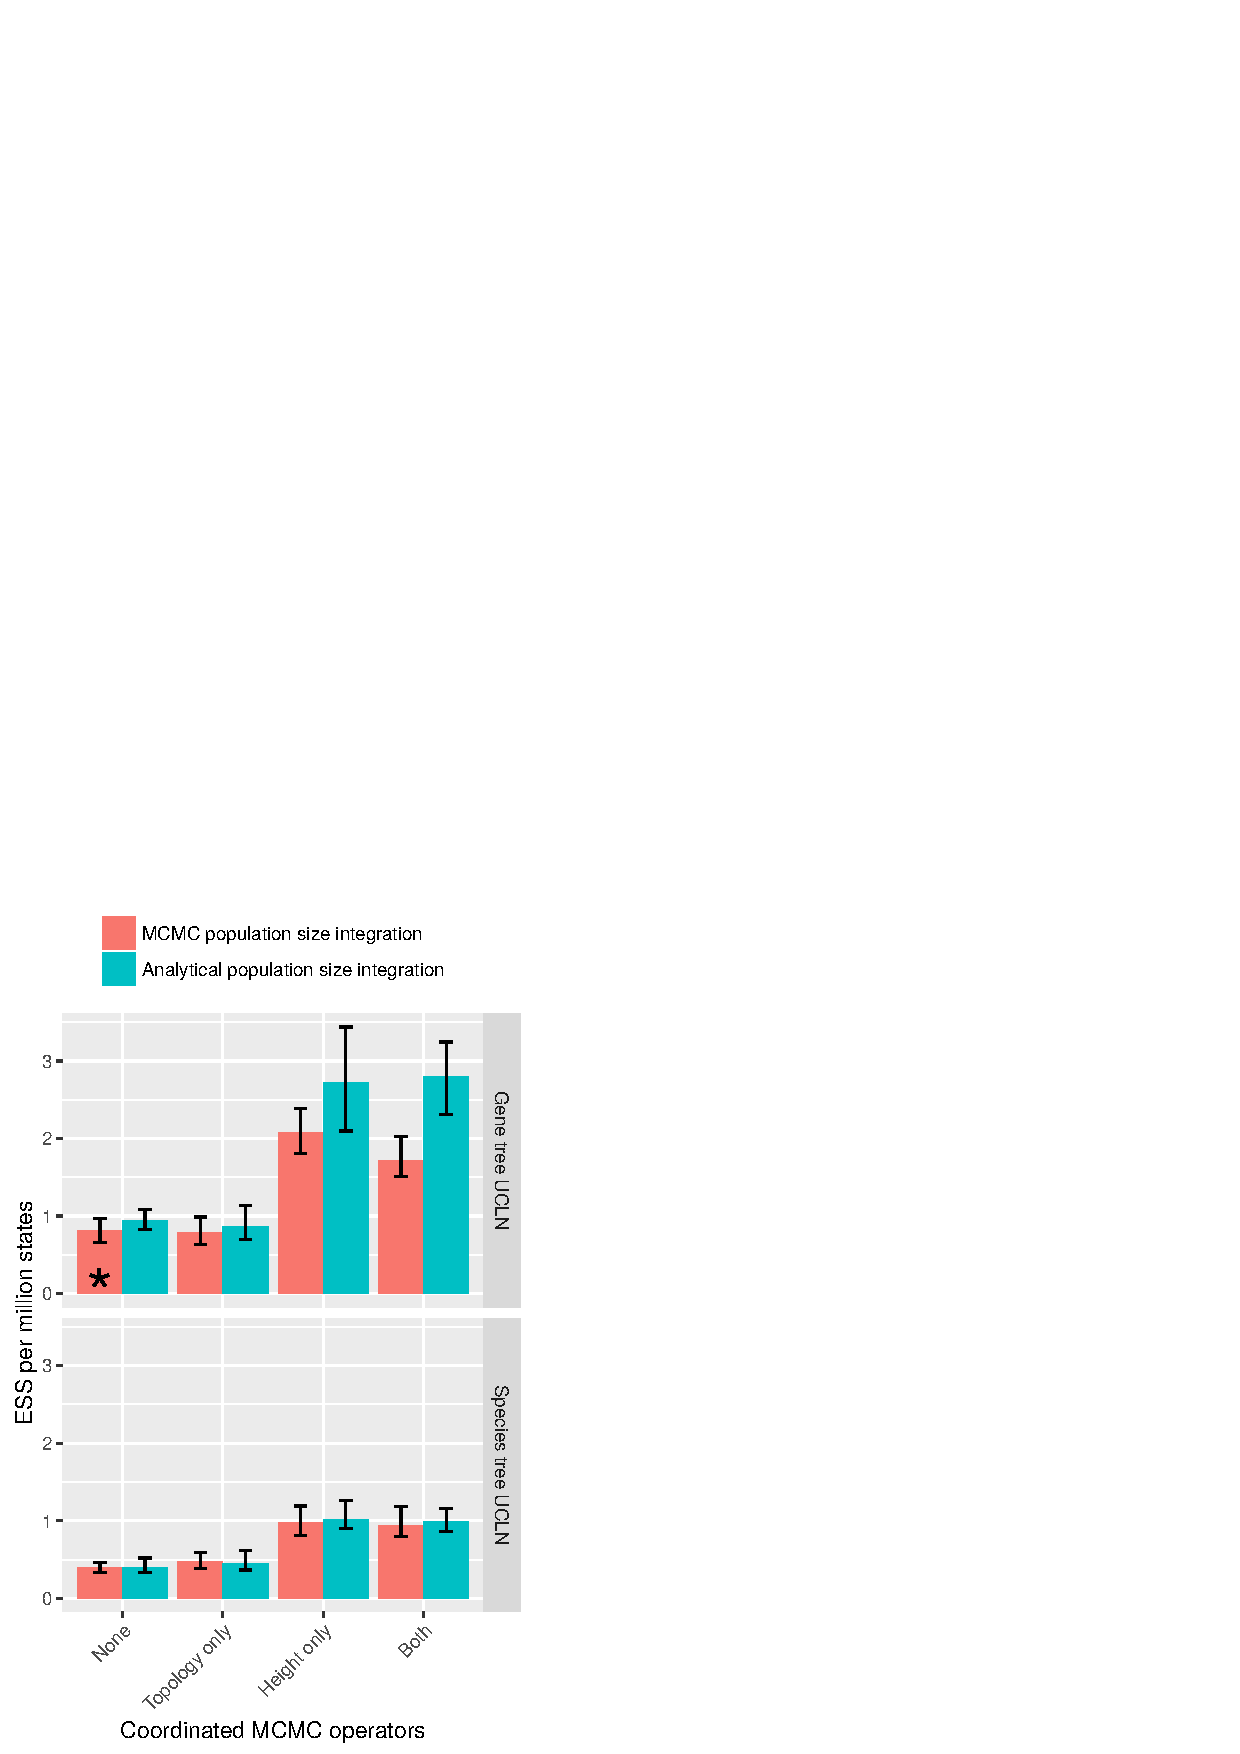
\includegraphics[height=14cm]{speciesTreeHeight_ess_per_mstates.pdf}
\caption
{Mean estimated sample size (ESS) per million states of the \textit{Pseudacris} species tree height.}
\label{fig:realEssPerMstates}
\end{figure}

\clearpage

\begin{figure}[htb!]
\centering
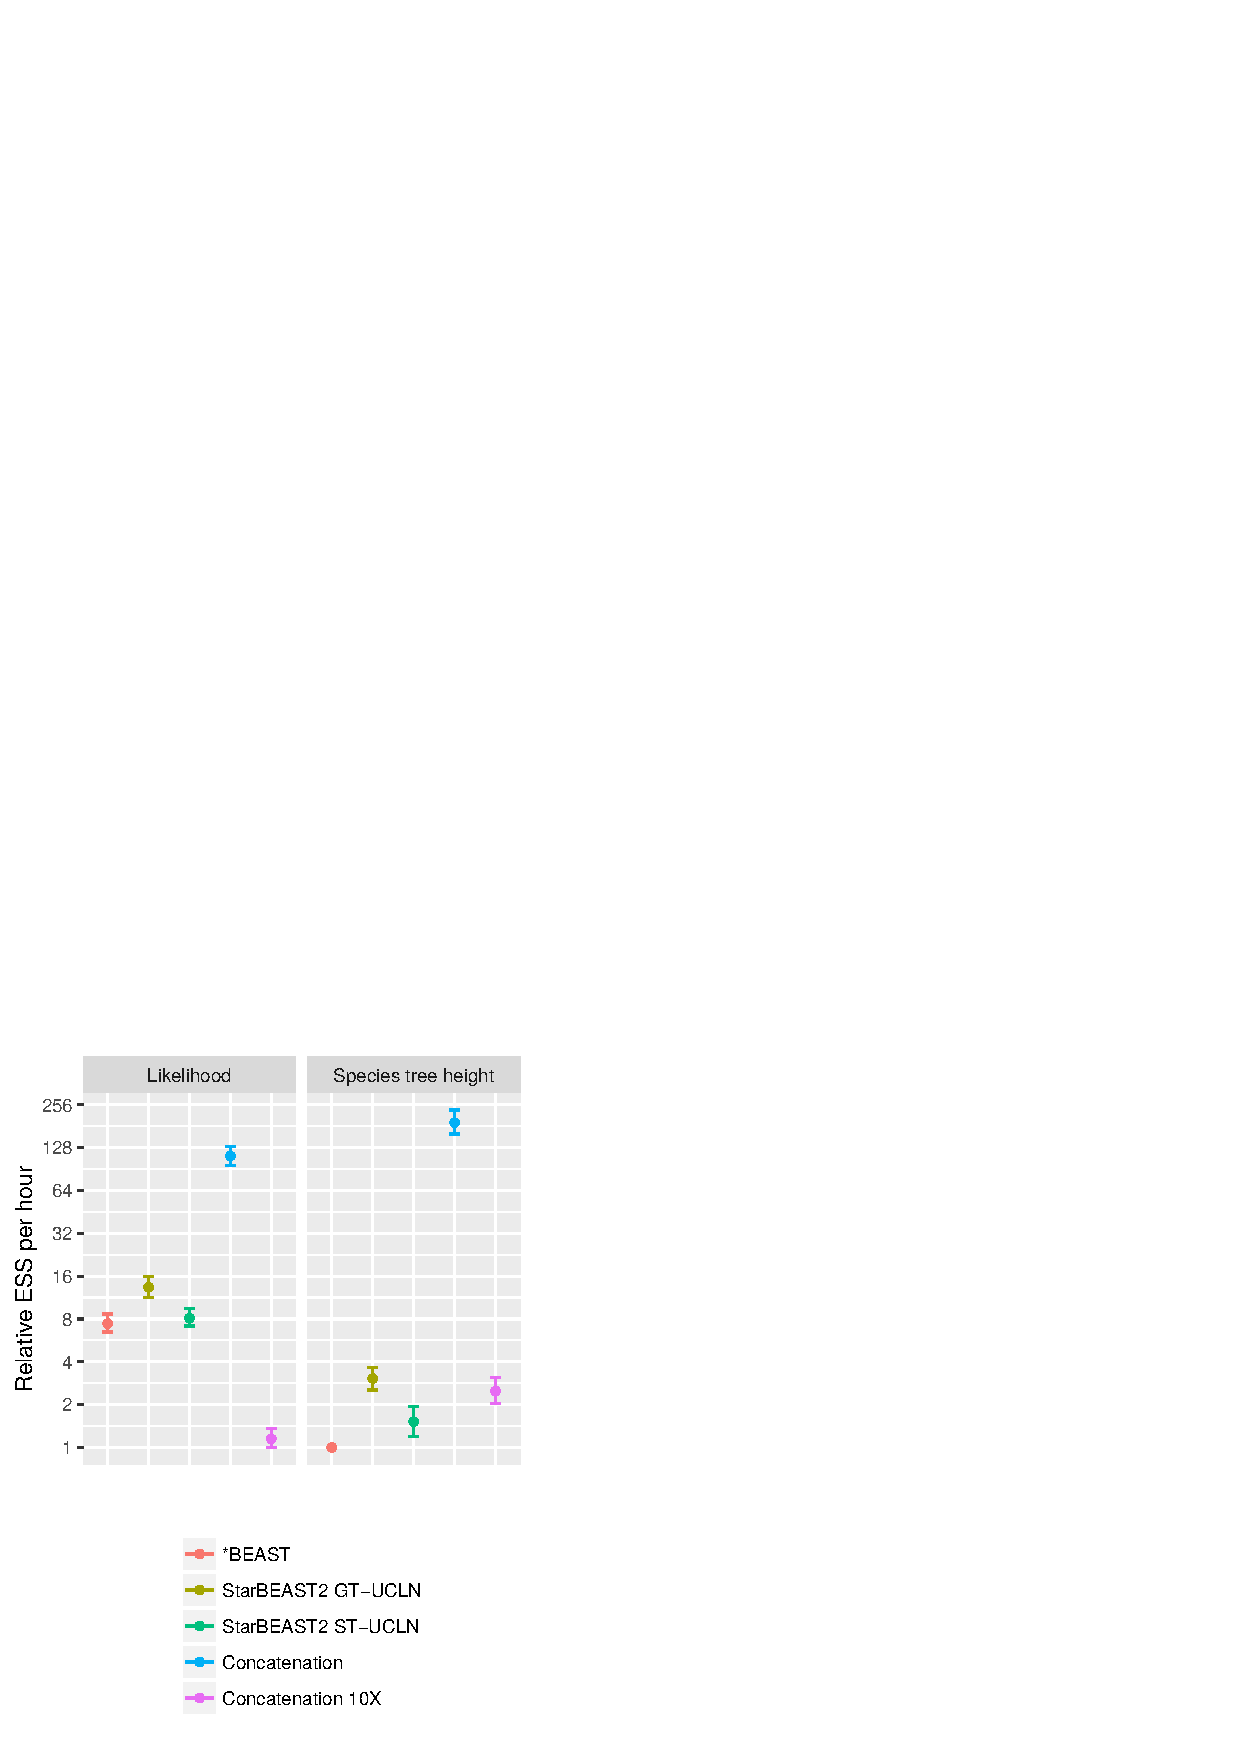
\includegraphics[width=16cm]{multiple_ess_per_hour.pdf}
\caption
{Convergence of different methods applied to simulated data. Methods are
concatenation with 22 loci, concatenation with 220 loci (10X), StarBEAST2 with
*BEAST settings and 22 loci, and StarBEAST2 with performant settings, 22 loci,
and uncorrelated lognormal relaxed clocks applied to the gene tree (GT-UCLN) or
to the species tree (ST-UCLN). Relative ESS per hour is the trimmed mean of
estimated sample size per hour for each replicate divided by the slowest rate
--- that of the species tree height estimated by StarBEAST2 with *BEAST
settings. Trimmed means (25\% trim) were used to reduce the influence of
outliers. All error bars are 95\% confidence intervals calculated by
bootstrapping. N = 64.}
\label{fig:simulatedEssPerHour}
\end{figure}

\clearpage

\begin{figure}[htb!]
\centering
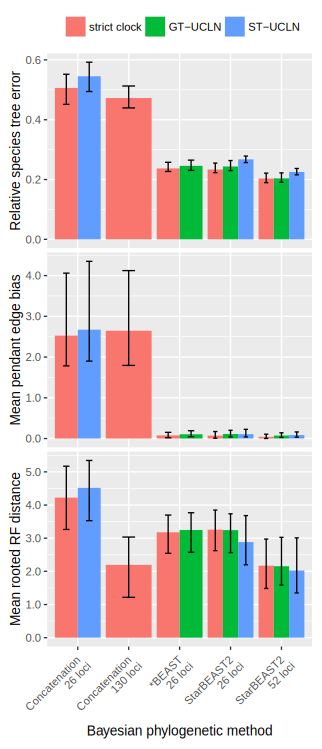
\includegraphics[width=6.5cm]{tree_error.pdf}
\caption
{Accuracy of different methods applied to simulated data. Methods are concatenation with 22 loci, concatenation with 220 loci
(10X), StarBEAST2 with *BEAST settings and 22 loci, and StarBEAST2 with
performant settings, 22 loci, and uncorrelated lognormal relaxed clocks applied
to the gene tree (GT-UCLN) or to the species tree (ST-UCLN). (A) Trimmed mean of
relative species tree error, a measure of branch length error. (B) Trimmed
mean of mean pendant edge bias, which measures biased estimates of the ages of
extant species. (C) Trimmed mean of mean rooted Robinson-Foulds distances, a
measure of topological error. Trimmed means (25\% trim) were used to reduce the
influence of outliers. All error bars are 95\% confidence intervals calculated
by bootstrapping. N = 64.}
\label{fig:speciesTreeError}
\end{figure}

\clearpage

\begin{figure}[htb!]
\centering
\includegraphics[width=16cm]{branch_rates_lm.pdf}
\caption
{Recovery of species tree branch rates using concatenation and StarBEAST2.
Methods are concatenation with 22 loci, concatenation with 220 loci (10X), and
StarBEAST2 with performant settings, 22 loci, and an uncorrelated lognormal
relaxed clocks applied to the species tree (ST-UCLN). Estimated rates are the
posterior expectation of the branch rate conditional on the monophyly of the
corresponding clade. $R^2$ values and lines of best fit were calculating using a separate
simple linear regression for each method. Root branch rates, which were fixed at
1.0, were excluded. N = 64.}
\label{fig:branchRatesLM}
\end{figure}

\clearpage

\section{Discussion}


\section{Materials and Methods}


\section{Supplementary Material}
Supplementary tables XX-XX and figures XX-XX are available at \textit{Molecular Biology and Evolution} online (http://www.mbe.oxfordjournals.org/).


\section{Acknowledgments}
Blah blah blah


\bibliographystyle{natbib}
\bibliography{starbeast2}

\end{document}
